\chapter{Introduction}\label{C:intro}

Test suites are becoming an increasing priority within software engineering development areas. Driven by agile methodologies incorporating practices such as test driven development and continuous integration. The use of a test suite is an attempt to cover the majority of situations that may occur. The number of situations is often endless, so covering the majority can incur a large number of tests and in turn take several hours to run. Throughout the project test cases are constantly being added, often when a piece of code is altered, new code is developed or a bug gets fixed. A question arises, how can we ensure that the first test case is not doing the same as the thousandth? Even with careful planning, it is near impossible to have no redundant test cases, which is when a test is nearly or exactly a replication of another test. Therefore, examination of the test cases should occur. 

During a tests execution, a 'paper trail' is left behind. This trail is the method executions that are called during the test, referred to as the tests spectra. A spectra is the set of data that will be analysed using different metrics to determine how related a test is with another. Each tests spectra will be analysed with every other test. Using this analysed information will help identify potential redundant test cases. In figure \ref{fig:spectra} we see the spectra's of three different tests. We clearly can see that Test 1 is different from Test 2 and 3. However, there appears to be similarities between Test 2 and 3 which may need further investigation.

\begin{figure}[h]
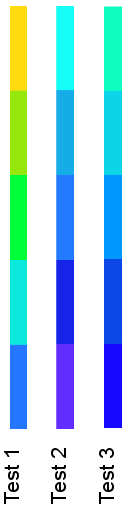
\includegraphics[width=3cm,height=6cm]{spectra.png}
\caption{Spectra}
\label{fig:spectra}
\end{figure}

It is important to understand the dangers of removing test cases. Unless two test cases are exactly the same, it is difficult to guarantee that they are indeed redundant, even if one is a subset of another. Therefore the aim of the project is to identify different approaches that give developers an idea on the number of redundant test cases that are contained within a project. It should allow the developer to run a set of pipelines they specify and view the results on a GUI, allowing manual inspection to determine if they are truly redundant. This means that the tool is useful for gaining an overview and understanding of the condition of the current test suite.

A potential use of the tool is to allow for splitting of any redundant tests into separate test suites allowing for them to be run at different times. For example, one test suite can be run during continuous integration, and the other over night. Ensuring that we are not losing any probability of finding a bug, instead redistributing the test time.

Dr David Pearce is currently writing a language called Whiley, which contains an extended static checking framework in order to eliminate run time exceptions through formal verification techniques. In the compiler module alone, there are roughly 40,000 tests. To reduce this number could result in allowing David Pearce to increase development speed due to a reduction in the time taken to run a large test suite. 